\documentclass[11pt]{article}
\usepackage{geometry}
\geometry{a4paper, margin=1in}
\usepackage{graphicx}
\usepackage{listings}
\usepackage{xcolor}
\usepackage[utf8]{inputenc}

\lstset{
    basicstyle=\ttfamily\small,
    breaklines=true,
    frame=single,
    language=C++,
    keywordstyle=\color{blue},
    commentstyle=\color{green!50!black},
    stringstyle=\color{red}
}

\title{Operating Systems Lab Assignment: Thread-Safe Data Structures}
\author{Christian Clarke}
\date{\today}

\begin{document}

\maketitle

\section{Introduction}
This report covers thread-safe data structures implemented in C++. Mutexes ensure safe concurrent access.

% =====================
\section{Exercise 1: Queue and Stack}
\lstinputlisting{thread_safe_data_structures.cpp}

\textbf{Explanation:} Mutexes and lock\_guard protect shared data.

\textbf{Analysis:} Prevents race conditions in producer-consumer and undo-redo.

\begin{figure}[h]
\centering
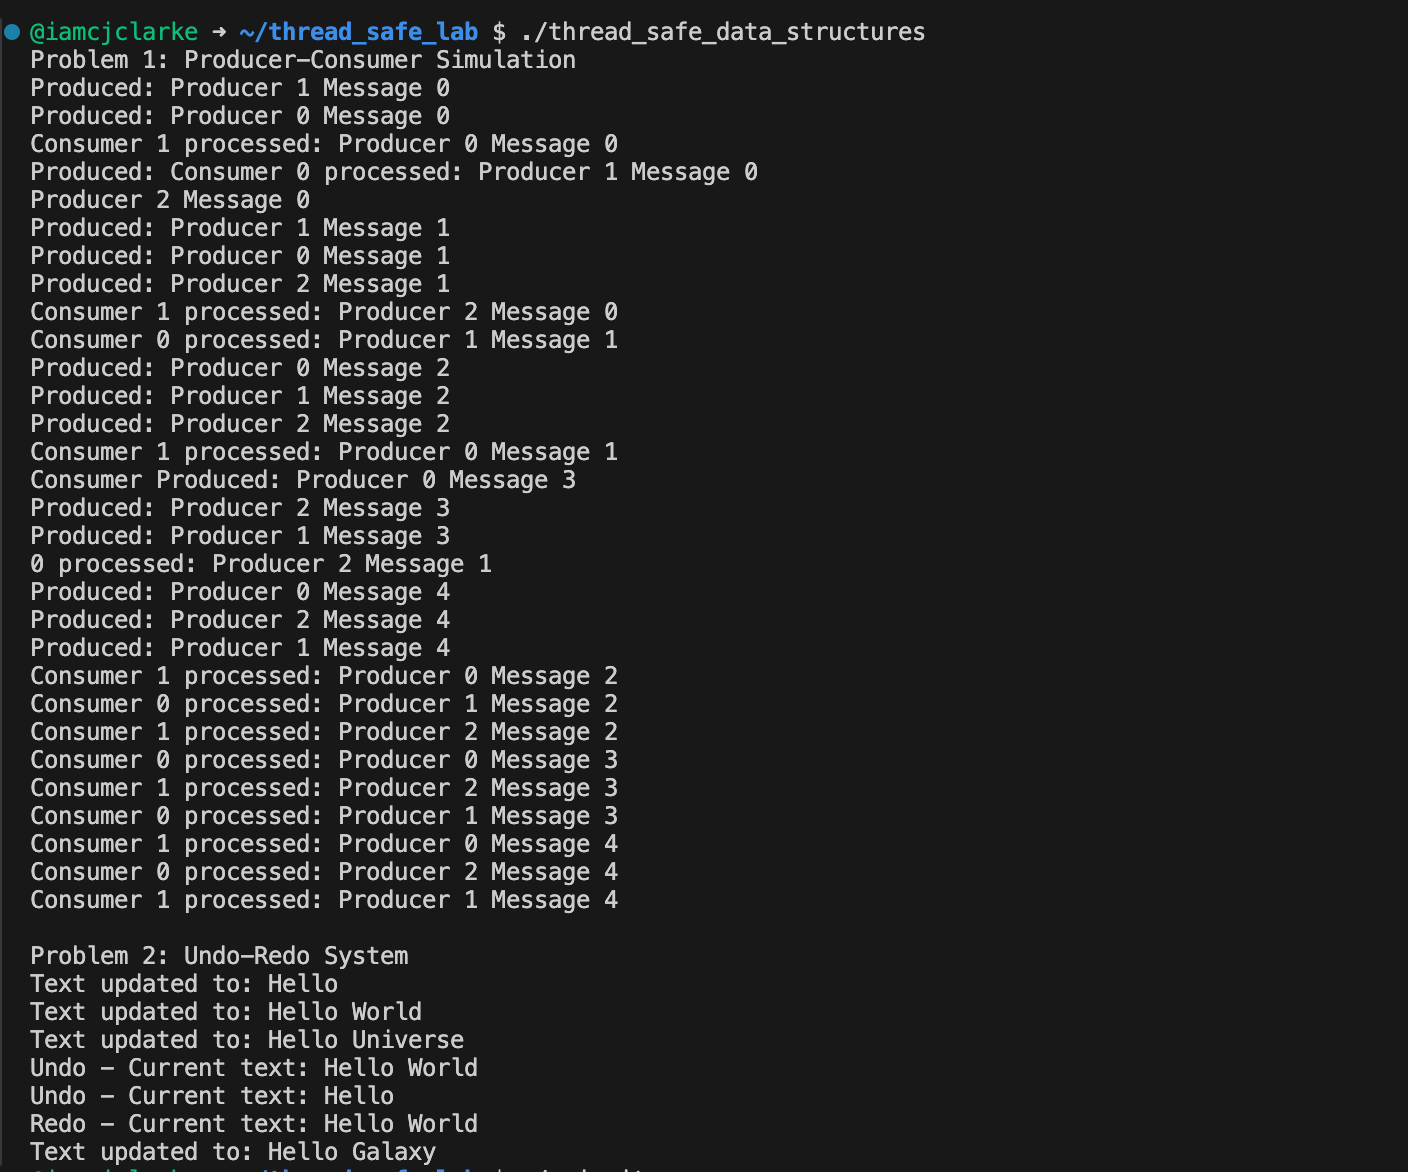
\includegraphics[width=\textwidth]{e1.png}
\caption{Exercise 1 Output}
\end{figure}

% =====================
\section{Exercise 3: Priority Queue}
\lstinputlisting{priority_queue.cpp}

\textbf{Explanation:} Thread-safe priority queue with multiple threads.

\textbf{Analysis:} Mutex ensures correct ordering and safe access.

\begin{figure}[h]
\centering
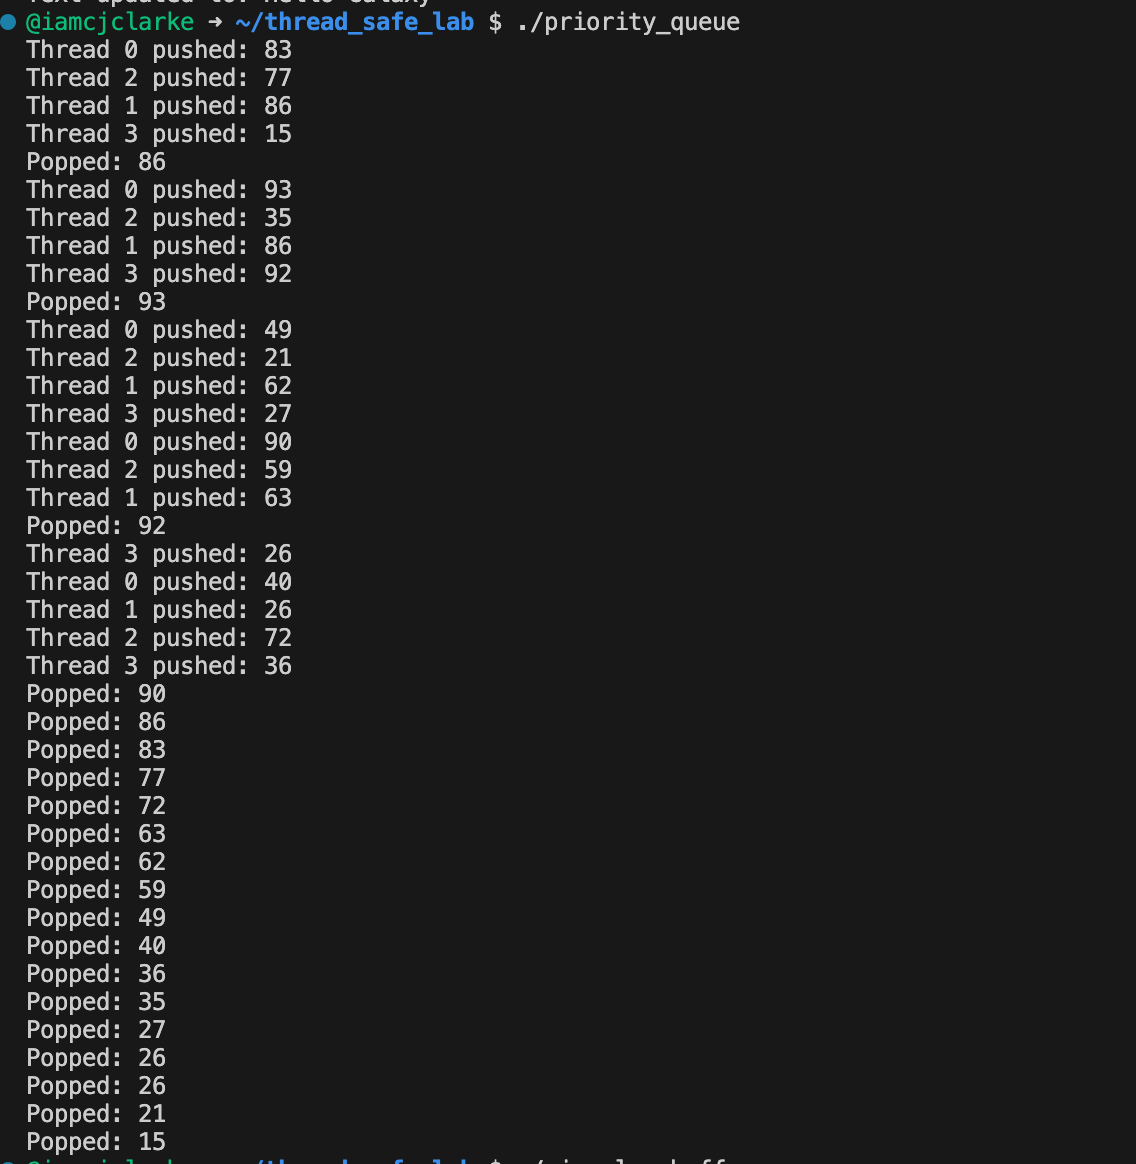
\includegraphics[width=\textwidth]{e3.png}
\caption{Exercise 3 Output}
\end{figure}

% =====================
\section{Exercise 4: Circular Buffer}
\lstinputlisting{circular_buffer.cpp}

\textbf{Explanation:} Uses condition variables for synchronization.

\textbf{Analysis:} Prevents overflow/underflow and avoids busy waiting.

\begin{figure}[h]
\centering
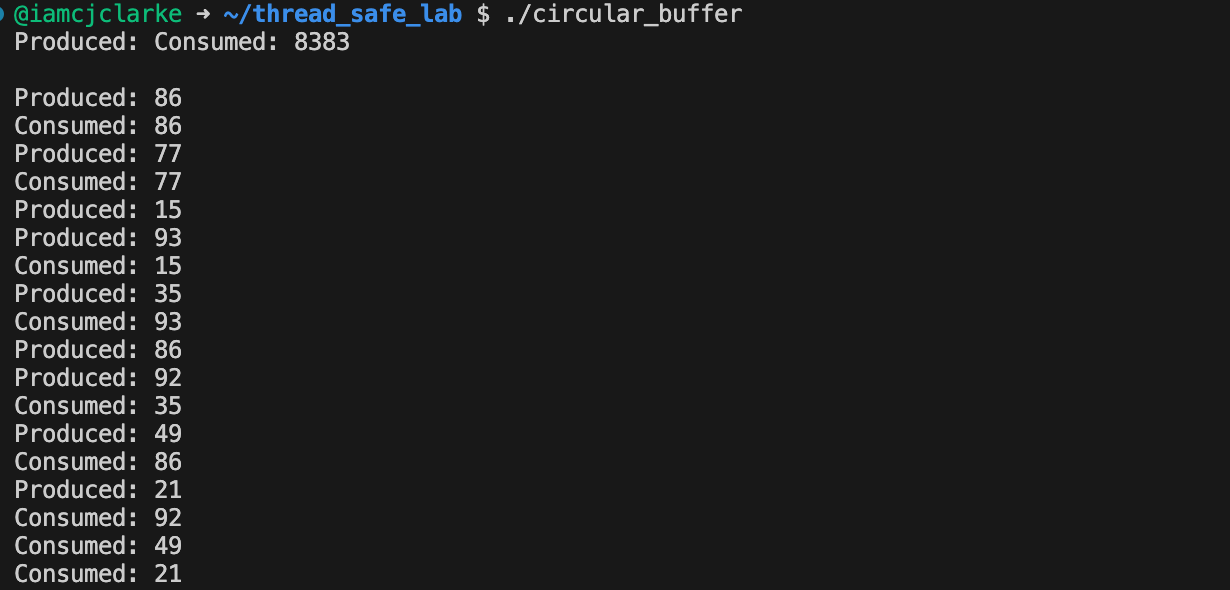
\includegraphics[width=\textwidth]{e4.png}
\caption{Exercise 4 Output}
\end{figure}

% =====================
\section{Exercise 5: Deque}
\lstinputlisting{thread_safe_deque.cpp}

\textbf{Explanation:} Supports thread-safe push/pop from both ends.

\textbf{Analysis:} Mutex ensures consistency when accessing both ends.

\begin{figure}[h]
\centering
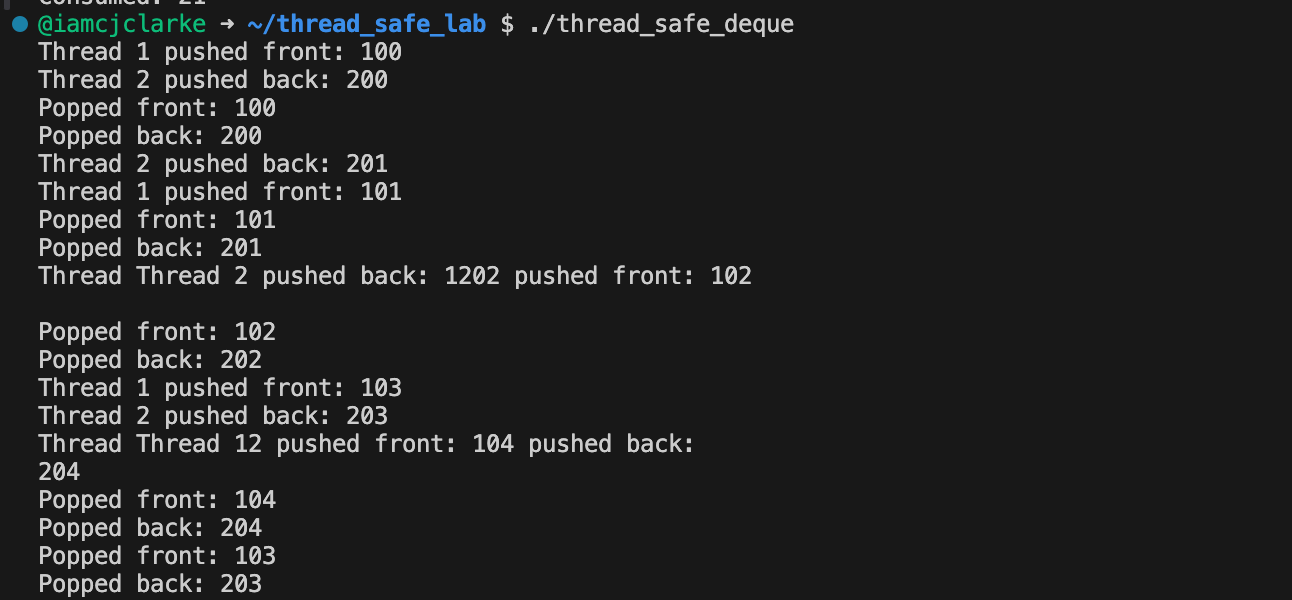
\includegraphics[width=\textwidth]{e5.png}
\caption{Exercise 5 Output}
\end{figure}

% =====================
\section{Exercise 6: Linked List}
\lstinputlisting{thread_safe_linked_list.cpp}

\textbf{Explanation:} Thread-safe singly linked list implementation.

\textbf{Analysis:} Mutex protects pointer updates to maintain list integrity.

\begin{figure}[h]
\centering
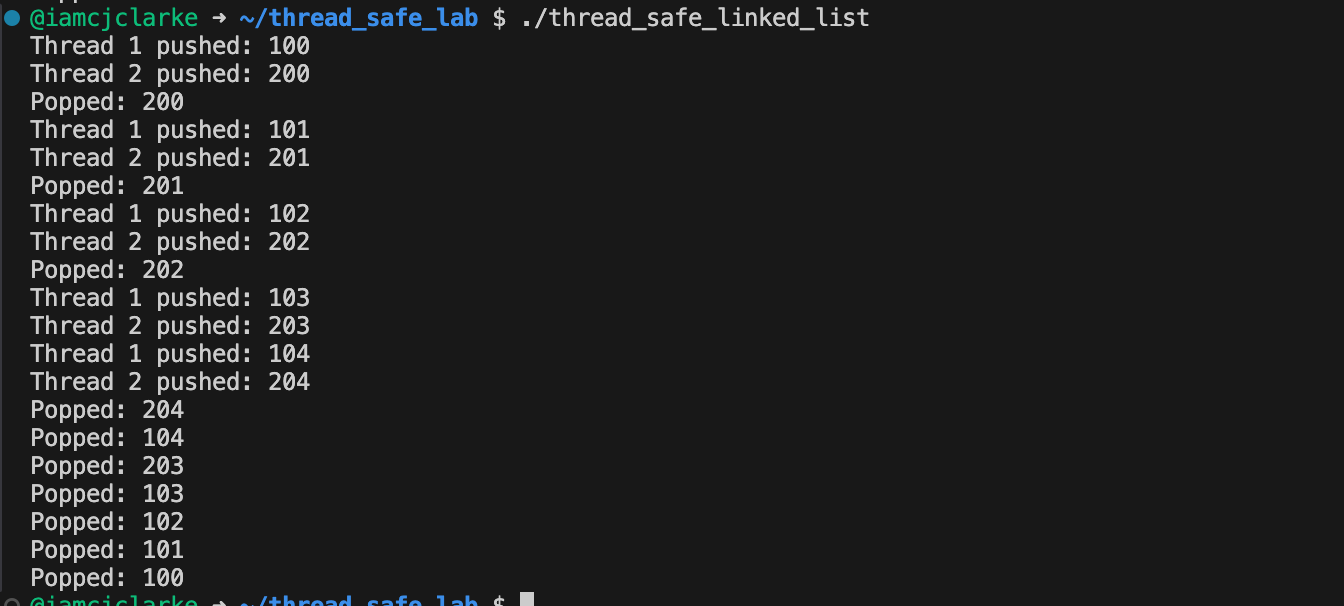
\includegraphics[width=\textwidth]{e6.png}
\caption{Exercise 6 Output}
\end{figure}

\end{document}
